%%%%%%%%%%%%%%%%%%%%%%%%%%%%%%%%%%%%%%%%%
% Beamer Presentation
% LaTeX Template
% Version 1.0 (10/11/12)
%
% This template has been downloaded from:
% http://www.LaTeXTemplates.com
%
% License:
% CC BY-NC-SA 3.0 (http://creativecommons.org/licenses/by-nc-sa/3.0/)
%
%%%%%%%%%%%%%%%%%%%%%%%%%%%%%%%%%%%%%%%%%

%----------------------------------------------------------------------------------------
%	PACKAGES AND THEMES
%----------------------------------------------------------------------------------------

\documentclass{beamer}

\mode<presentation> {

% The Beamer class comes with a number of default slide themes
% which change the colors and layouts of slides. Below this is a list
% of all the themes, uncomment each in turn to see what they look like.

%\usetheme{default}
%\usetheme{AnnArbor}
%\usetheme{Antibes}
%\usetheme{Bergen}
%\usetheme{Berkeley}
%\usetheme{Berlin}
%\usetheme{Boadilla}
%\usetheme{CambridgeUS}
%\usetheme{Copenhagen}
%\usetheme{Darmstadt}
%\usetheme{Dresden}
%\usetheme{Frankfurt}
%\usetheme{Goettingen}
%\usetheme{Hannover}
%\usetheme{Ilmenau}
%\usetheme{JuanLesPins}
%\usetheme{Luebeck}
\usetheme{Madrid}
%\usetheme{Malmoe}
%\usetheme{Marburg}
%\usetheme{Montpellier}
%\usetheme{PaloAlto}
%\usetheme{Pittsburgh}
%\usetheme{Rochester}
%\usetheme{Singapore}
%\usetheme{Szeged}
%\usetheme{Warsaw}

% As well as themes, the Beamer class has a number of color themes
% for any slide theme. Uncomment each of these in turn to see how it
% changes the colors of your current slide theme.

%\usecolortheme{albatross}
%\usecolortheme{beaver}
%\usecolortheme{beetle}
%\usecolortheme{crane}
%\usecolortheme{dolphin}
%\usecolortheme{dove}
%\usecolortheme{fly}
%\usecolortheme{lily}
%\usecolortheme{orchid}
%\usecolortheme{rose}
%\usecolortheme{seagull}
%\usecolortheme{seahorse}
%\usecolortheme{whale}
%\usecolortheme{wolverine}


\setbeamertemplate{navigation symbols}{} % To remove the navigation symbols from the bottom of all slides uncomment this line
}

\usepackage{graphicx} % Allows including images
\usepackage{booktabs} % Allows the use of \toprule, \midrule and \bottomrule in tables
\usepackage{amssymb}
\usepackage{amsmath}

\title[Automatic Metadata Extraction]{Automatic Metadata Extraction with Conditional Random Fields} % The short title appears at the bottom of every slide, the full title is only on the title page

\author{Joseph Boyd} % Your name
\institute[EPFL] % Your institution as it will appear on the bottom of every slide, may be shorthand to save space
{
\'Ecole Polytechnique F\'ed\'erale de Lausanne \\ % Your institution for the title page
\medskip
\textit{joseph.boyd@epfl.ch} % Your email address
}
\date{\today} % Date, can be changed to a custom date

\begin{document}

\begin{frame}
\titlepage % Print the title page as the first slide
\end{frame}

%------------------------------------------------

\section{Project Objectives}
\begin{frame}[noframenumbering]{Outline}
\tableofcontents[currentsection]
\end{frame}

%------------------------------------------------

\begin{frame}
\frametitle{Project Objectives}
\begin{itemize}
\item Take the existing state-of-the-art in metadata extraction and optimise it for HEP papers
\item We will use Conditional Random Fields (CRFs) to build a probabilistic model
\item CRFs combine ideas from log linear models (logistic regressions) and hidden Markov models (HMMs)
\end{itemize}
\end{frame}

%------------------------------------------------

\section{Theory}
\begin{frame}[noframenumbering]{Outline}
\tableofcontents[currentsection]
\end{frame}

%------------------------------------------------

\subsection{Logistic Regression}
\begin{frame}
\frametitle{Logistic Regression}
\begin{itemize}
\item A logistic regression is used for classifying a data sample into two (binary) or more (multi) categories, thus,
$$\hat{\text{y}}_{prediction} = \boldsymbol\beta^{T} \cdot \boldsymbol{x}_{sample},$$
where $\hat{y}$ is the prediction (represented as a probability), $\boldsymbol{x} = [x_0, x_1, ..., x_D]^T$ is a data sample, and $\boldsymbol\beta = [\beta_0, \beta_1, ..., \beta_D]^T$ is the vector of parameters we must \emph{learn}
\item We construct a (maximum log likelihood) cost function in terms of this parameter vector,
$$\mathcal{L}(\boldsymbol\beta) = \sum_{n=1}^N y_n\boldsymbol\beta^T\boldsymbol{x}_n - \log[1 + \exp(\boldsymbol\beta^T\boldsymbol{x}_n)]$$
\end{itemize}
\end{frame}

%------------------------------------------------

\begin{frame}
\frametitle{Solving a Logistic Regression}\begin{itemize}
\item Building a regression model is equivalent to solving a convex optimisation problem (i.e. maximising the cost function)
\item We know the form of the model, and we have a set of (training) data
\item We want to choose the model parameters for which the error is minimised (think line of best fit)
\item We use a numerical method to find the global minimum of error, for example, the method of gradient descent:
$$\boldsymbol\beta^{k+1} = \boldsymbol\beta^{k} - \alpha\nabla\mathcal{L}(\boldsymbol\beta^{k})$$
\end{itemize}
Take home message: we can automatically build mathematical functions for making predictions
\end{frame}

%------------------------------------------------

\subsection{Hidden Markov Models}
\begin{frame}
\frametitle{Hidden Markov Models (HMMs)}
\end{frame}

%------------------------------------------------

\begin{frame}
\frametitle{Hidden Markov Models (HMMs) - Example}
\end{frame}

%------------------------------------------------

\begin{frame}
\frametitle{Solving Hidden Markov Models}
\begin{itemize}
\item Solved using dynamic programming techniques
\end{itemize}
Take home message: once we have the model, we can make predictions for a given input \emph{efficiently}.
\end{frame}

%------------------------------------------------

\subsection{Conditional Random Fields}
\begin{frame}
\frametitle{Conditional Random Fields (CRFs)}
\end{frame}

% ------------------------------------------------

\section{Grobid}
\begin{frame}[noframenumbering]{Outline}
\tableofcontents[currentsection]
\end{frame}

%------------------------------------------------

\begin{frame}
\frametitle{Grobid}
\begin{itemize}
\item Grobid (GeneRation Of BIbliographic Data) is a Java-based tool for managing CRF models 
\item It coordinates the training and usage of a ``cascade'' of models, computed with a CRF engine backend
\end{itemize}
\begin{figure}[!ht]
\center
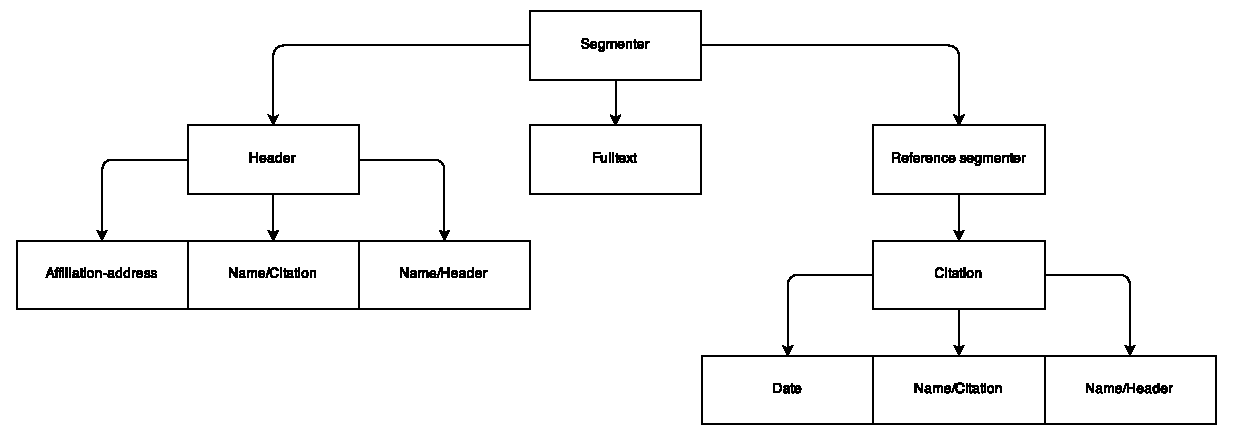
\includegraphics[width=4in]{figures/cascade.pdf}
\caption{Cascade of models used by Grobid}
\label{fig:cascade}
\end{figure}
\end{frame}

%------------------------------------------------

\begin{frame}
\frametitle{Grobid - Details}
\end{frame}

%------------------------------------------------

\section{Initial Results}
\begin{frame}[noframenumbering]{Outline}
\tableofcontents[currentsection]
\end{frame}

%------------------------------------------------

\begin{frame}
\frametitle{Initial Results}
\end{frame}

%------------------------------------------------

\section{Next Steps}
\begin{frame}[noframenumbering]{Outline}
\tableofcontents[currentsection]
\end{frame}

%------------------------------------------------

\begin{frame}
\frametitle{Next Steps}
\end{frame}

%------------------------------------------------

\end{document} 